\chapter{Einf�hrung}
	
	\section{Projektteam}
	
		\begin{figure}[H]
    \centering
    \begin{minipage}[b]{0.48\textwidth}
        \centering
        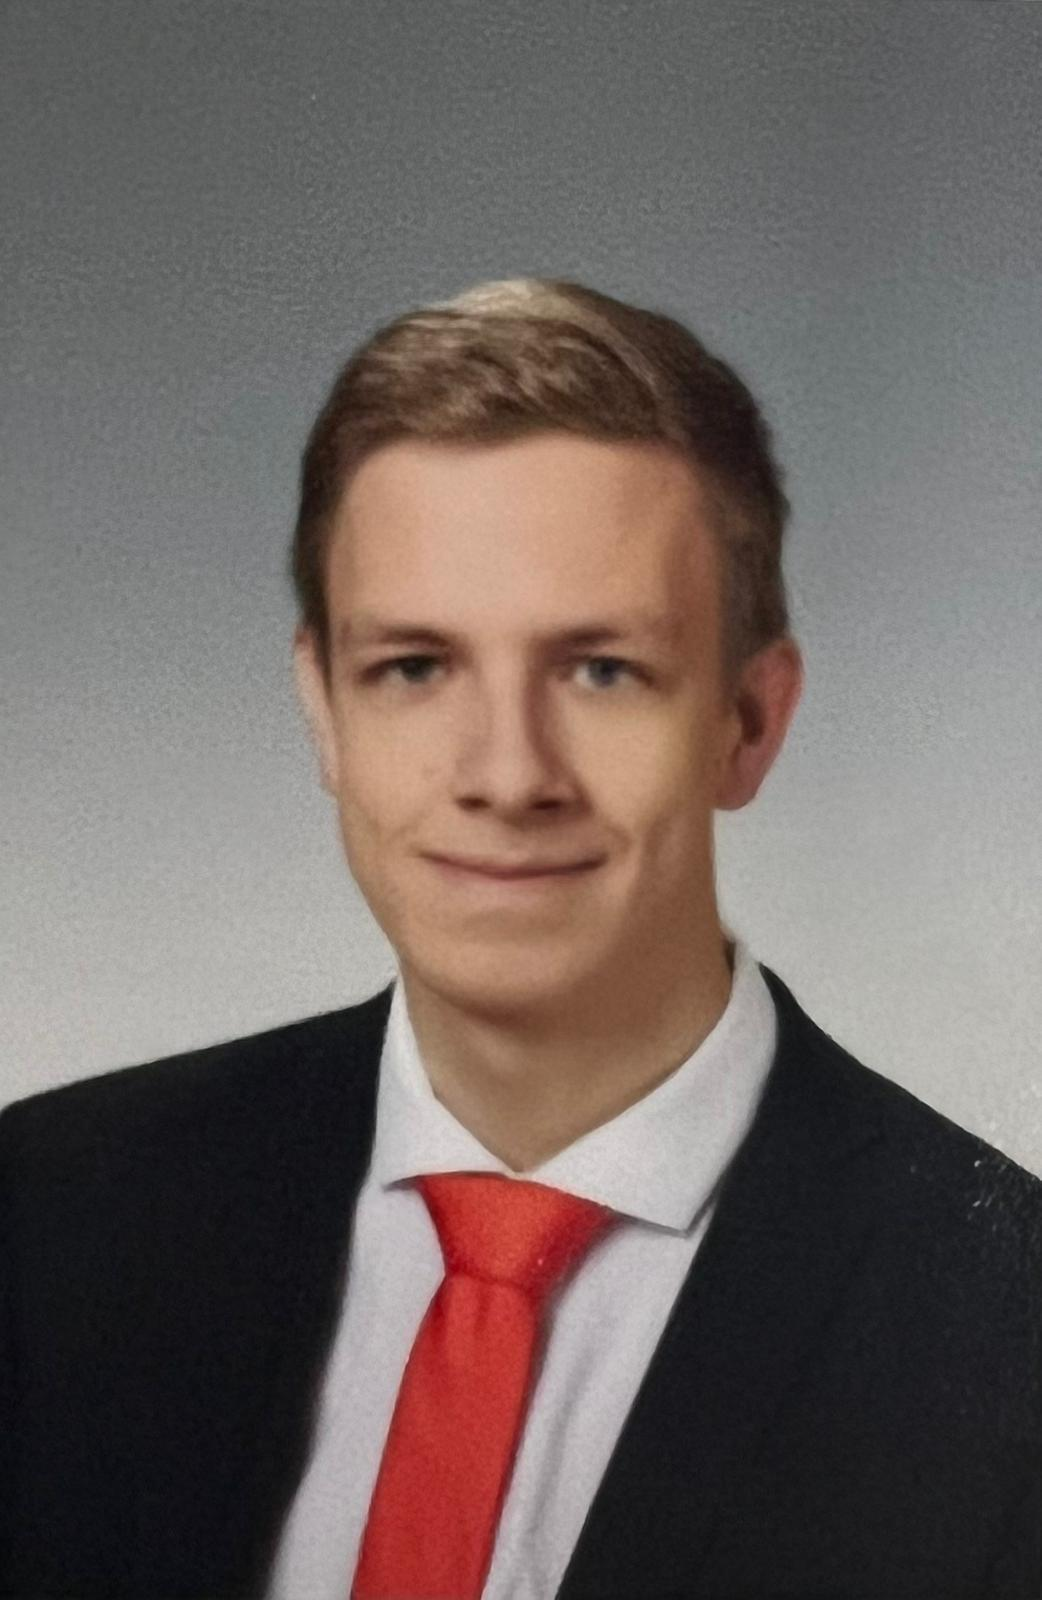
\includegraphics[scale=0.12]{./1_Einfuehrung/Abbildungen/Felix}
        \caption{Felix Sandri}
    \end{minipage}
    \begin{minipage}[b]{0.48\textwidth}
        \centering
        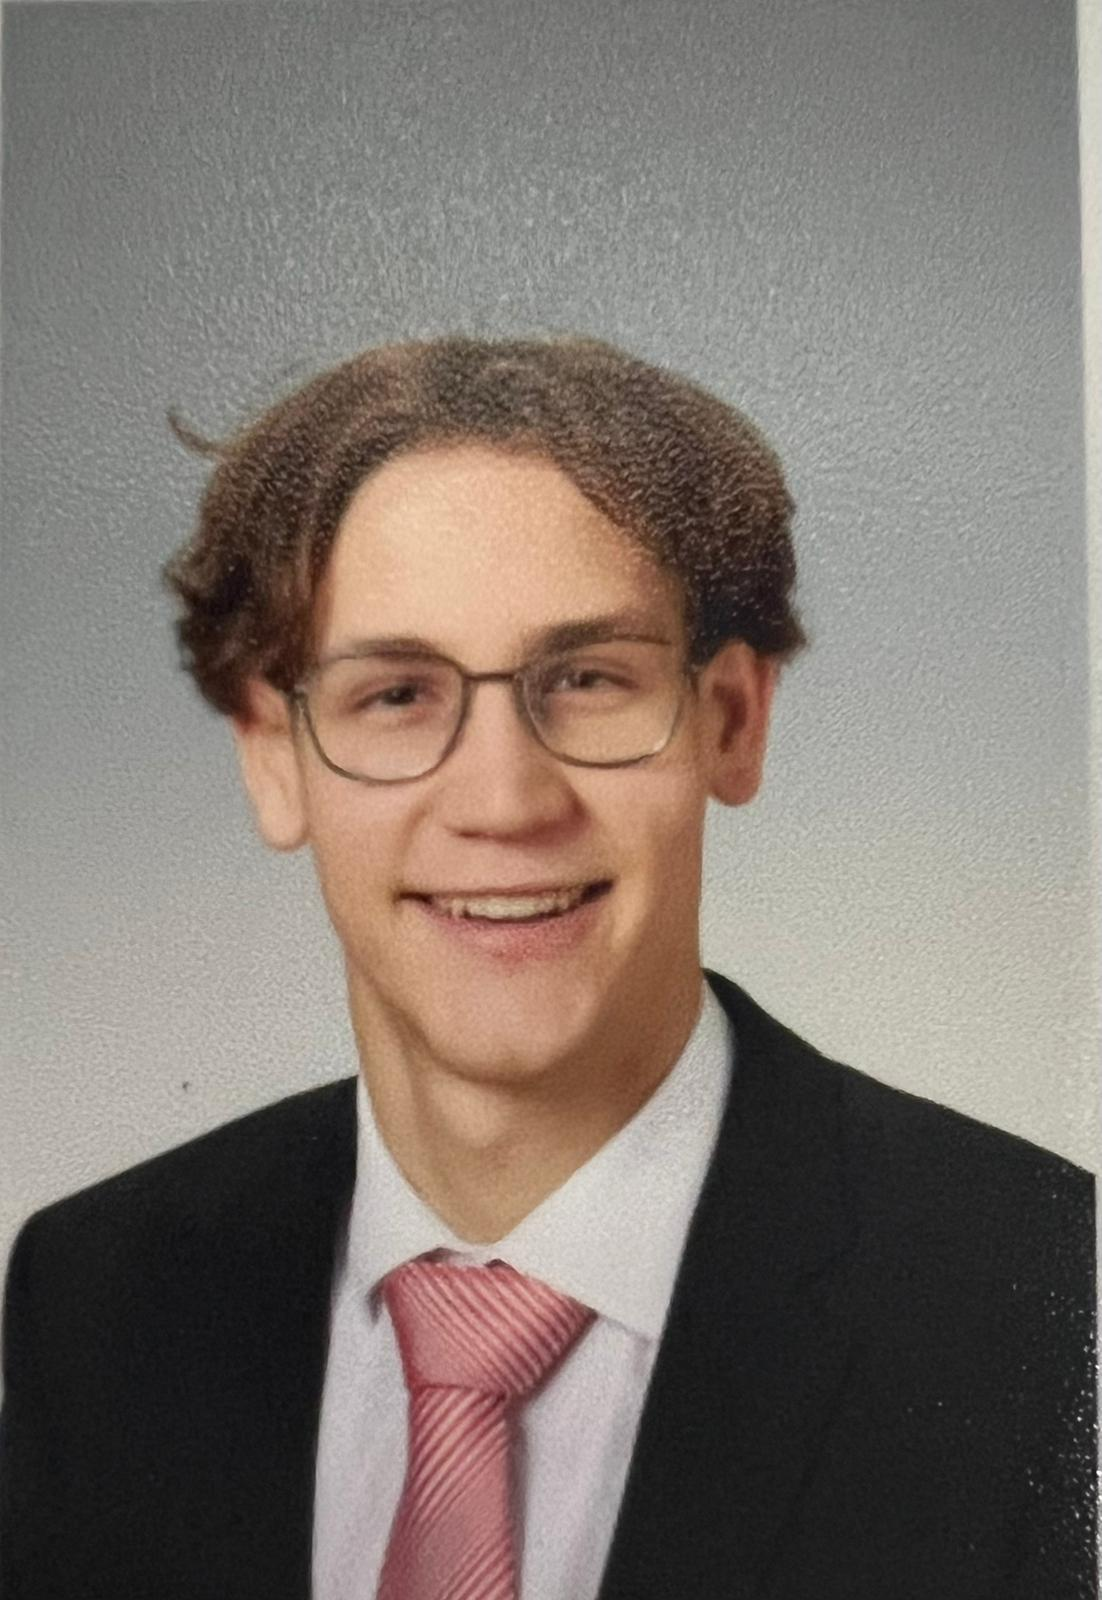
\includegraphics[scale=0.12]{./1_Einfuehrung/Abbildungen/Philipp}
        \caption{Philipp Kaltenleitner}
    \end{minipage}
	\end{figure}
	\begin{figure}[H]
    \centering
    \begin{minipage}[b]{0.48\textwidth}
        \centering
        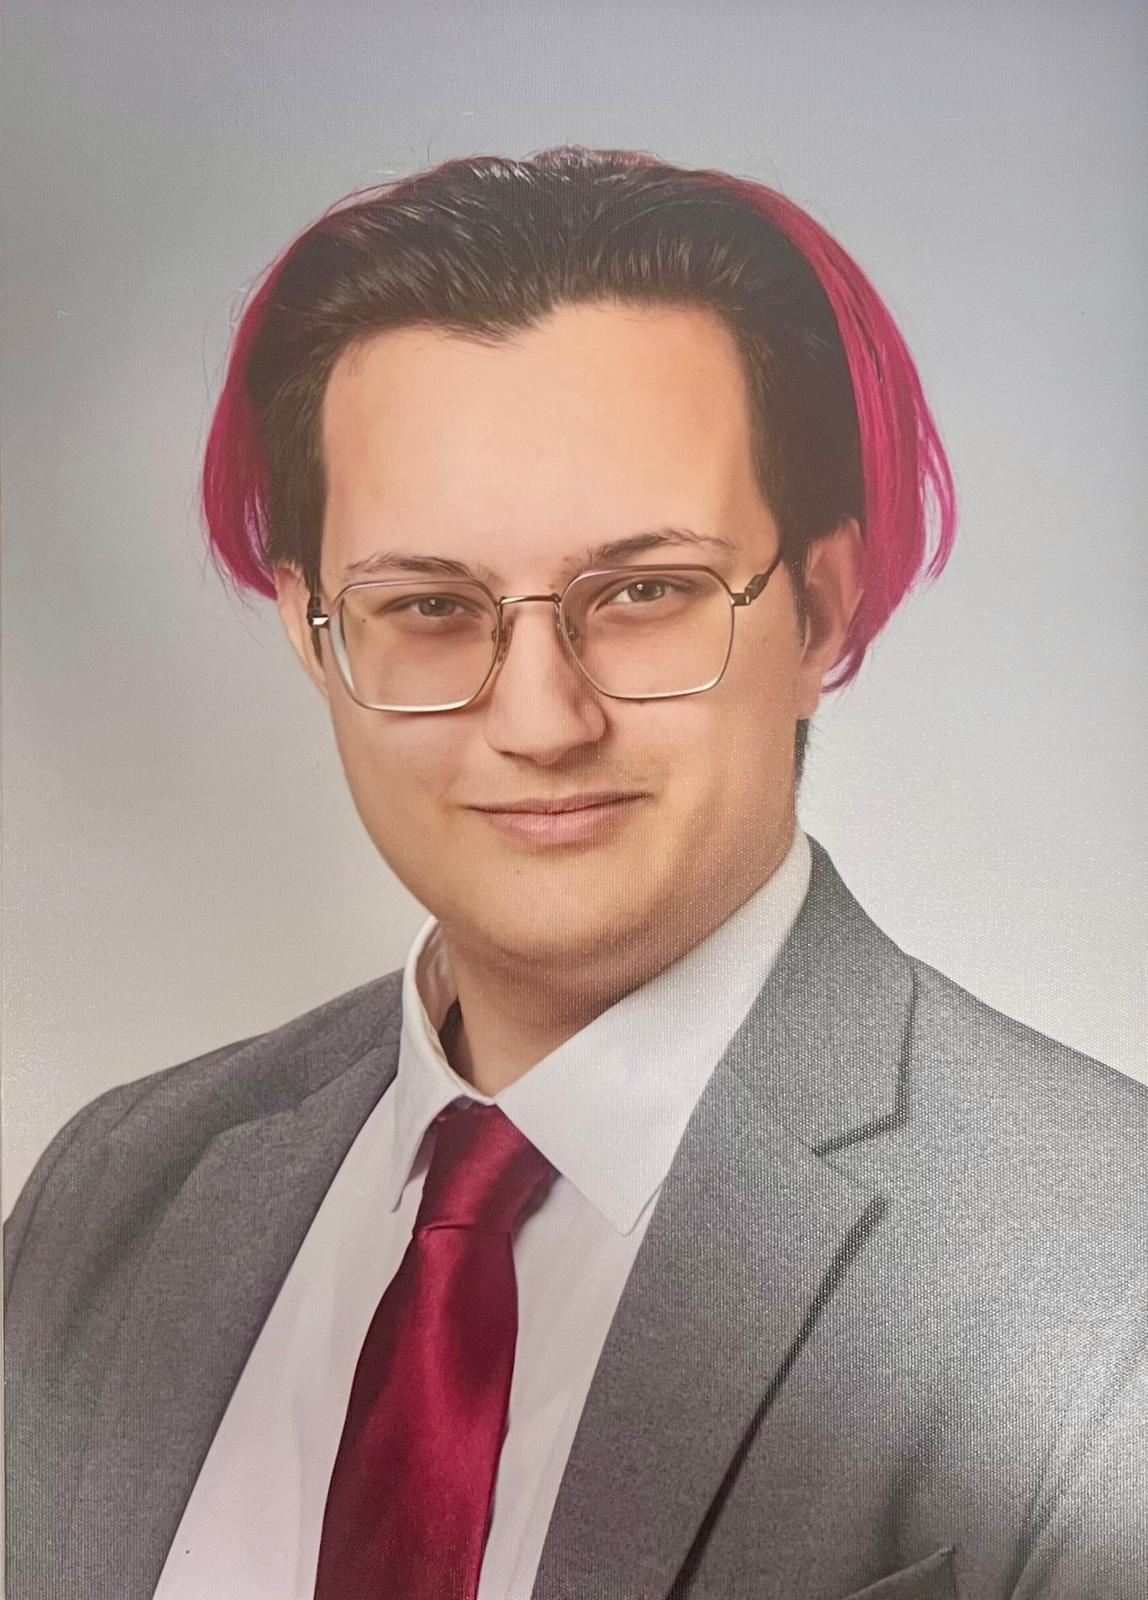
\includegraphics[scale=0.12]{./1_Einfuehrung/Abbildungen/Mert}
        \caption{Mert G�kay G�rel}
    \end{minipage}
    \begin{minipage}[b]{0.48\textwidth}
        \centering
        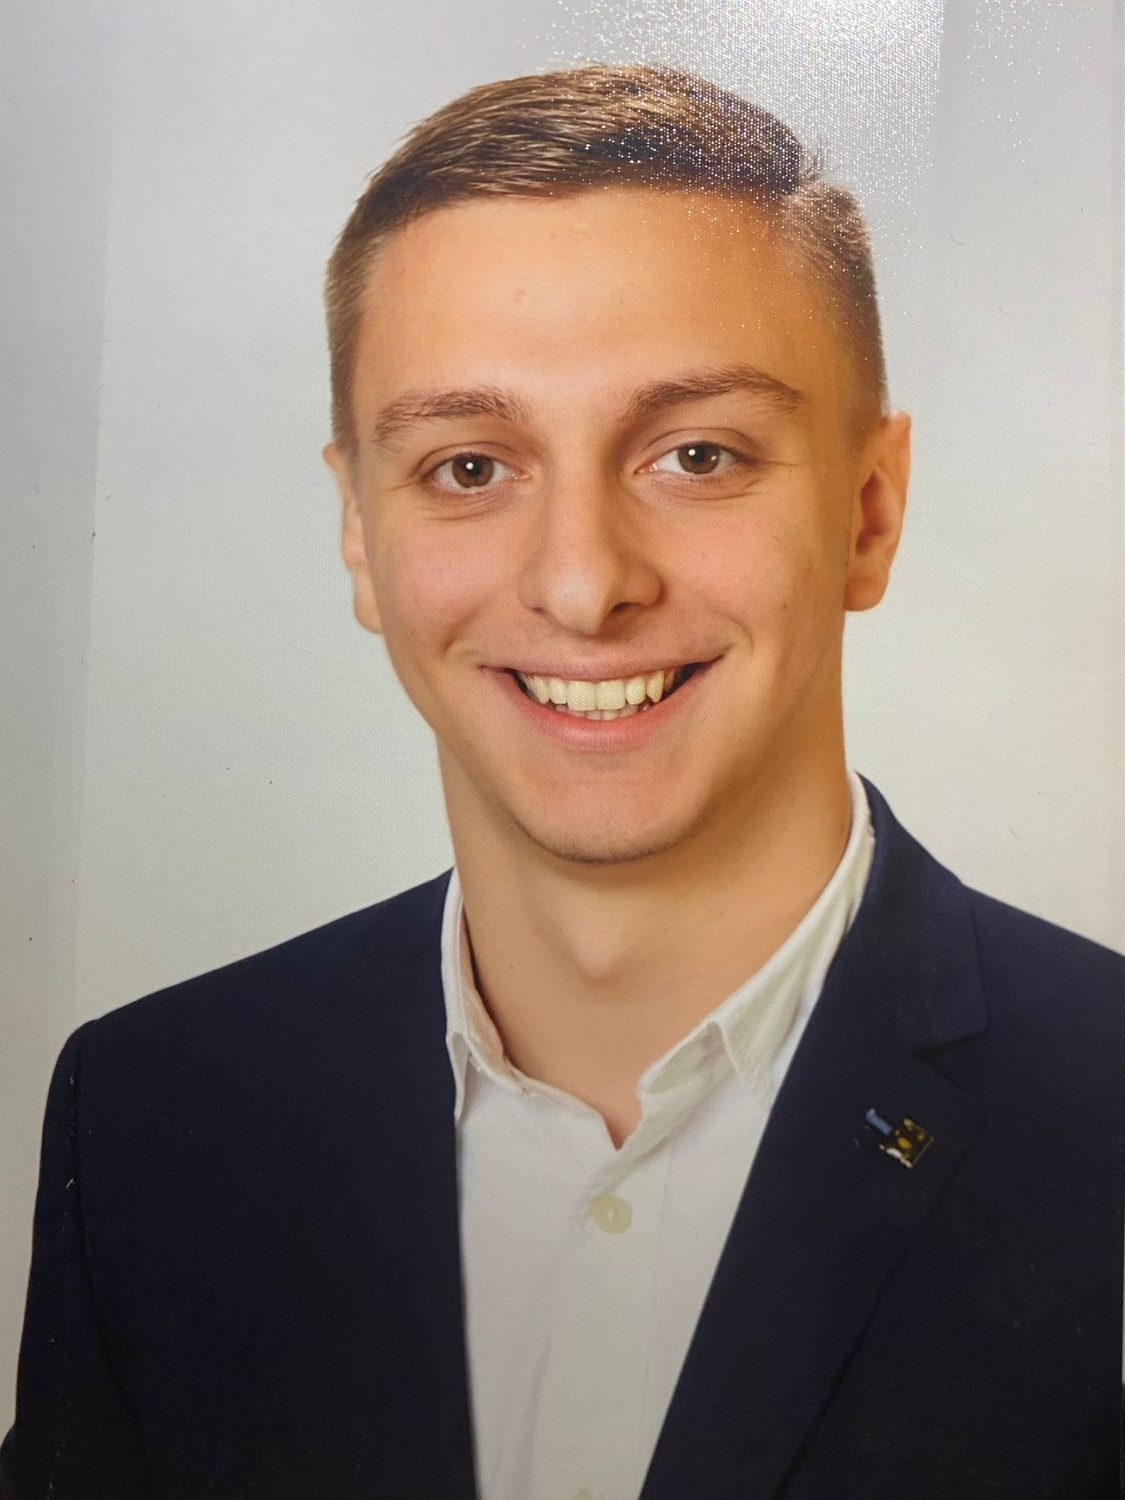
\includegraphics[scale=0.12]{./1_Einfuehrung/Abbildungen/David}
        \caption{David Petrovic}
    \end{minipage}
	\end{figure}
\newpage

\section{Projektbetreuer}
	\begin{itemize}
		\item \textbf{Prof. Dipl.-Ing. Robert Fuchs} unterst�tzte Felix Sandri beim fertigen und implementieren des elektrischen Antriebssystems.
		\item \textbf{Prof. Dipl.-Ing. Reinhold Benedikter} war stets eine gro�e Unterst�tzung w�hrend dem gesamten Verlauf des Projekts, er half beim Bestellen aller Komponenten und unterst�tzte Philipp Kaltenleitner erheblich beim �berarbeiten der Aufh�ngung und Lenkung.
		\item \textbf{BSc Simon Dantendorfer} unterst�tzte Mert G�rel bei Fragen bez�glich Optimierung der Software und Implementierung der ROS-Entwicklungsumgebung.
		\item \textbf{Prof. Dipl.-Ing. Timo Huemer} betreute David Petrovic bez�glich der Vorgehensweise w�hrend der Softwareentwicklung und dem Designprozess der Website.
	\end{itemize}

\section{Aufgabenteilung}